\documentclass{standalone}
\usepackage{tikz}
\usetikzlibrary{shapes.misc, arrows.meta, positioning, bending}

%% Helper: pill-shaped node label -- a filled dot followed by a monospaced name.
%% Usage inside a [station] node: \stlabel{NODE\_ID}
\newcommand{\stlabel}[1]{\textbullet\enspace\texttt{#1}}

\begin{document}
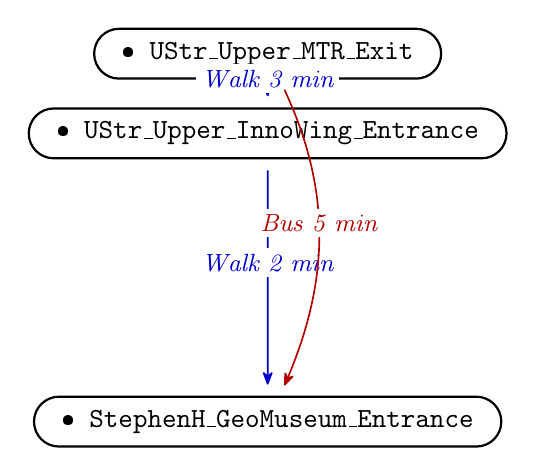
\begin{tikzpicture}[
    %% -- Node styles ------------------------------------------------------
    %%
    %% station: pill/stadium shape (semi-circular ends, like a metro map).
    %%   Use \stlabel{NAME} as the node content to get the dot + monospaced text.
    %%   Example:
    %%     \node[station] (A) {\stlabel{MTR\_A2}};
    station/.style={
        draw,
        shape=rounded rectangle,   % from shapes.misc -- true semi-circular ends
        rounded rectangle arc length=180,
        minimum height=1.8em,
        inner xsep=0.9em,
        align=center,
        thick,
        fill=white,
    },
    %% -- Base directed edge style ------------------------------------------
    %%
    %%   All per-solution styles inherit from this.
    %%   For parallel edges use bend left/right:
    %%     \draw[sol1, bend left=20] (A) to node[elabel, above] {label} (B);
    route/.style={
        ->,
        >=Stealth[round],
        semithick,
        shorten >=4pt,
        shorten <=4pt,
    },
    %% -- Per-solution edge styles (one colour per solution) ----------------
    %%
    %%   Usage:  \draw[sol1] (A) -- (B);
    %%           \draw[sol2, bend left=20] (A) to node[elabel, above] {text} (B);
    sol1/.style={route, color=blue!80!black},           % Solution 1 -- blue
    sol2/.style={route, color=red!70!black},            % Solution 2 -- red
    sol3/.style={route, color=green!55!black},          % Solution 3 -- green
    sol4/.style={route, color=orange!85!black},         % Solution 4 -- orange
    sol5/.style={route, color=violet!80!black},         % Solution 5 -- violet
    %% -- Edge label style -------------------------------------------------
    %%
    %%   Place inline on an edge:
    %%     \draw[sol1] (A) -- node[elabel, above] {5 min / Walk} (B);
    elabel/.style={font=\small\itshape, inner sep=2pt, fill=white},
]

%% -- Place nodes here -----------------------------------------------------

\node[station]                                          (UStr_Upper_MTR_Exit) {\stlabel{UStr\_Upper\_MTR\_Exit}};
\node[station, below=10pt of UStr_Upper_MTR_Exit]        (UStr_Upper_InnoWing_Entrance) {\stlabel{UStr\_Upper\_InnoWing\_Entrance}};
\node[station, below=3cm of UStr_Upper_InnoWing_Entrance]       (StephenH_GeoMuseum_Entrance) {\stlabel{StephenH\_GeoMuseum\_Entrance}};

%% -- Draw edges here ------------------------------------------------------

%% Solution 1 (blue):
\draw[sol1] (UStr_Upper_MTR_Exit) -- node[elabel, above] {Walk 3 min} (UStr_Upper_InnoWing_Entrance);
\draw[sol1] (UStr_Upper_InnoWing_Entrance) -- node[elabel, above] {Walk 2 min} (StephenH_GeoMuseum_Entrance);

% Solution 2 (red) -- offset with bend to avoid overlapping sol1:
\draw[sol2, bend left=25] (UStr_Upper_MTR_Exit) to node[elabel, above] {Bus 5 min} (StephenH_GeoMuseum_Entrance);

\end{tikzpicture}
\end{document}